\large{
\section{Definizioni preliminari}
Di seguito andremo a definire le varie nozioni preliminari che dovranno essere ben note e delucidate prima di poter proseguire con la definizione di grafo clusterizzato. Le seguenti definizioni non hanno l'obiettivo di chiarire e delucidare a pieno il lettore riguardo gli argomenti trattati ma sono definizioni e spunti per poter definire almeno in minima parte l'ambito di studio su cui si andrà a sviluppare il lavoro svolto e anticipazioni per quanto concerne la struttura dati creata su cui l'editor andrà a lavorare.

\subsection{Grafi}
%%inserire disegno grafo qui
\begin{figure}[!htb]
	\begin{center}
		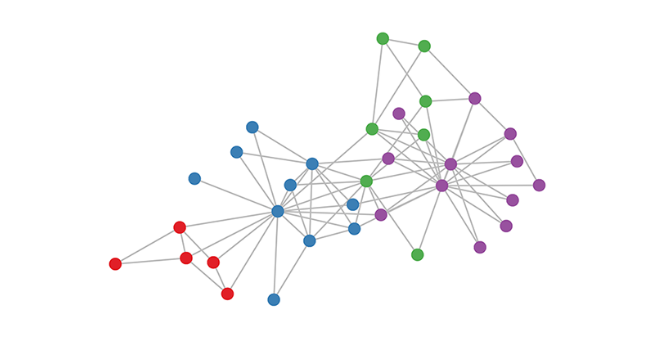
\includegraphics[width=0.7 \linewidth]{figure/grafoGenerico}
	\end{center}
	\caption{Esempio di grafo indiretto connesso \label{fig:grafoGenerico}}
\end{figure}

Un grafo G è definito da una coppia di insiemi \textbf{$<V,E>$} in cui V è un insieme di nodi o vertici che possono essere connessi tra loro mediante l'insieme di archi E tale che i suoi elementi siano coppie di elementi dell'insieme V esprimibile come $$E \subseteq V * V$$ \\
Si definisce poi grafo \textbf{completo} un grafo in cui ogni vertice è collegato con tutti gli altri vertici rimanenti di modo che l'insieme degli archi E è esplimibile come $E= V * V$.
Dato un grafo è possibile avere un disegno $\tau(G)$ come mapping dei vertici su punti distinti del piano.
Data la definizione di grafo è necessario ,ai fini di una introduzione al mondo della teoria dei grafi ed in particolare a quello dei grafi clusterizzati, enunciare la definizione di grafo \textbf{planare}.\\
Un grafo\textbf{ planare }nella teoria dei grafi è definito come un grafo che può essere raffigurato in un piano in modo che non si abbiano archi che si intersecano. È facile da intuire che non tutti i grafi sono planari, e se ne riportano due famosi esempi in \textbf{\figurename~\ref{fig:kuratowski}}
%%inserire qui figure di grafi planari e dei grafi di kuratowski
\begin{figure}[!htb]
	\begin{center}
		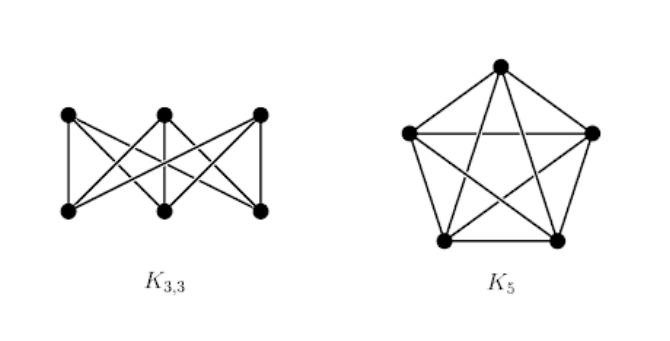
\includegraphics[width=0.9 \linewidth]{figure/kuratowski}
	\end{center}
	\caption{grafi di Kuratowski \label{fig:kuratowski}}
\end{figure}
\newline
In particolare questi due grafi sono chiamati anche grafi di Kuratowski mediante i quali si può dare la definizione di grafo Planare anche come enunciato del \textit{\textbf{Teorema di Kuratowski}}:
\begin{center}
\textit{	Un grafo è planare \textit{se e solo se} non contiene alcun sottografo che sia una espansione di $K_5 $ o una espansione di $K_3,_3$\\}
\end{center}
Si ricorda inoltre che se un grafo è planare allora ammette un disegno planare $\tau(G)$. Dando un altra definizione si può evidenziare che un disegno $\tau(G)$ è un disegno planare ogni arco non interseca nulla eccetto i due vertici che connette. Si richiama inoltre all'algoritmo di Auslander e Parter del 1961. Mediante questo algoritmo del costo non lineare a livello di complessità computazionale ma uguale a $O(n^3)$ si è in grado di calcolare se un grafo in input è planare o meno ed è possibile formulare il seguente teorema
\begin{center}
	\textit{un grafo è un planare se il suo disegno è sempre colorabile con 4 colori diversi}
\end{center}
Questo è un punto chiave nella teoria dei grafi quando poi si andrà a discutere dei grafi clusterizzati poco più avanti.
I grafi risultano comunque essere una delle strutture fondamentali su cui si basano molte applicazioni reali.
\subsection{Alberi}
\begin{figure}[!htb]
	\begin{center}
		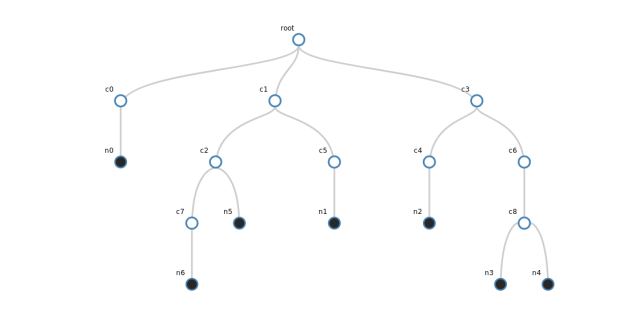
\includegraphics[width=0.8 \linewidth]{figure/alberoGenerico}
	\end{center}
	\caption{esempio di albero n-ario \label{fig:alberoGenerico}}
\end{figure}
Data la definizione di grafo si può dunque definire un albero \textbf{tree} come un grafo connesso non orientato e senza cicli come mostrato in \textbf{\figurename~\ref{fig:alberoGenerico}}. Per essere tale quindi il grafo in questione o deve possedere un solo cammino per ogni coppia di vertici oppure essere aciclico massimale.
Ogni nodo appartenente ad un albero possiede un livello dato alla somma $ 1 + L(padre) $ intendendo che la radice dell'albero ha livello 0.\\
La radice è definita come l'unico nodo dell'albero che non possiede archi entranti ma solo archi uscenti e a cui solitamente viene data rappresentazione del livello più basso dell'albero in altre parole è l'unico nodo che non presenta nodi con livello inferiore(i nodi padri) ma solo nodi con livello superiore(i nodi figli). 
I nodi dell'albero diversi dalla radice possono inoltre essere partizionati in due categorie:\\
\begin{itemize}
	\item\textbf{nodi interni} definiti come nodi con almeno un figlio e suddivisibili ulteriormente in nodi bassi in cui tutti i figli sono foglie e nodi alti che possiedono almeno un figlio nodo interno;
	\item\textbf{foglie }che non possiedono figli e per questo non hanno archi uscenti.
\end{itemize}

\begin{figure}[!htb]
	\begin{center}
		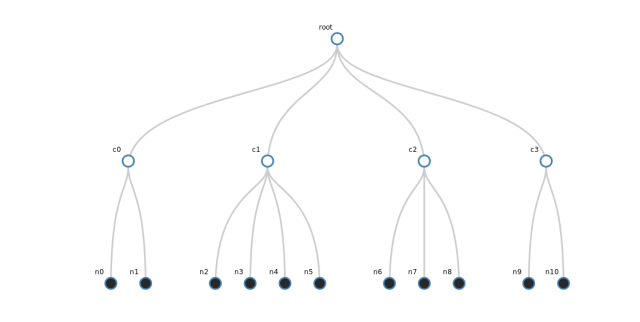
\includegraphics[width=0.8 \linewidth]{figure/flatTree}
	\end{center}
	\caption{esempio di flat Tree \label{fig:flatTree}}
\end{figure}
Un nodo è inoltre definibile \textbf{omogeneo} se tutti i figli di quel nodo sono foglie o sono nodi interni.
Data la definizione di nodo omogeneo, viene detto che un albero è omogeneo se e solo se tutti i suoi nodi sono nodi omogenei.
Date queste definizioni introduttive relative agli alberi è possibile definire un albero flat (come mostrato in \textbf{\figurename~\ref{fig:flatTree}}) come un albero in cui tutte le sue foglie hanno profondità pari a due.\\
Definendo in questo modo un albero flat è facile notare come ogni albero flat è anche omogeneo avendo tutti i nodi interni che hanno come figli esclusivamente foglie ed il nodo radice che possiede solo nodi interni come figli.\\
Per completezza si voglio dare anche le definizioni di profondità di un nodo e di altezza di un albero rispettivamente come la lunghezza del cammino dalla radice al nodo e la profondità massima dei suoi nodi.
Una volta terminate le definizioni iniziali si può proseguire con quella di grafo clusterizzato.
\section{C-Graph}
\begin{figure}[!htb]
	\begin{center}
		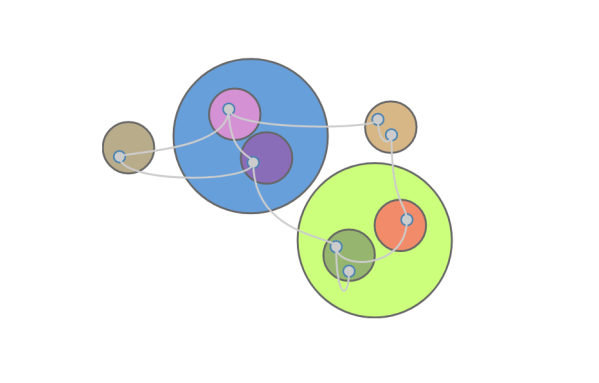
\includegraphics[width=0.9 \linewidth]{figure/cgraphGenerico}
	\end{center}
	\caption{esempio di grafo clusterizzato \label{fig:cgraphGenerico}}
\end{figure}
Un grafo clusterizzato (\textbf{c-graph}),di cui ne è un esempio la \textbf{\figurename~\ref{fig:cgraphGenerico}}, è definito come un grafo \textbf{planare} con una gerarchia ricorsiva definita sui suoi vertici. In altre parole un \textit{c-graph} C è definito come $$C=<\textbf{G},\textbf{T}>$$ 
Ovvero come una coppia $<G,T>$ dove:
\begin{itemize}
	\item\textbf{$G=(V,E)$} è un grafo planare, formato quindi da nodi e da archi le cui rappresentazioni non intersecano nulla se non il punto iniziale e finale, definito come \textit{underlying graph} di C;
	\item\textbf{$T$} è un albero radicato definito come \textit{inclusion tree} in cui l'insieme delle foglie di T coincide con l'insieme dei nodi V dell'underlying graph $G$ ed ogni nodo interno è rappresentato da un \textbf{cluster}.
\end{itemize}
Un cluster in informatica può essere definito come un insieme di oggetti simili spesso connessi tra loro a cui al suo interno può contenere altri sotto cluster.
Nel caso specifico del termine infatti si denota che un cluster potrà quindi contenere altri cluster al suo interno e/o nodi dell'insieme $V$ dell'Underlying graph $G$.
Un cluster essendo un nodo dell'albero dovrà quindi avere una "conoscenza" del nodo precedente(genitore) e dei nodi successivi(figli) 
Per quanto riguarda la struttura dati quella sarà analizzata con più consapevolezza nei capitoli successivi in cui verranno elencate e motivate scelte di progetto partendo dalle definizioni date ora.
\subsection{clustered planarity}
Avendo definito la struttura c-graph C si può andare ad analizzare come si comporta per quanto concerne il disegno $\tau(C)$. 
Avendo definito l'underlying graph come un grafo planare si devono fare delle considerazioni per quanto riguarda il disegno dell'intero C-graph.\\
Questo disegno sarà un disegno planare \textbf{c-planar} se:\\
\begin{itemize}
	\item[(i)] ogni cluster è rappresentato da una singola regione del piano che contiene solo i suoi vertici e gli archi a cui essi sono collegati;
	\item[(ii)] definendo il perimetro del cluster come bordo del cluster, si ha che un disegno sarà planare se nessun bordo del disegno $\tau$(c-graph) si interseca con altri bordi di altri cluster;
	\item[(iii)] ogni arco si interseca con un cluster al più una volta;
\end{itemize}
Per ciò che concerne la teoria dell'informatica e dei grafi, i problemi relativi alla planarità e al disegno planare di grafi clusterizzati risultano essere ancora di grande importanza e oggetto di molte ricerche in quanto ancora non si è in grado di definire la complessità del decidere quando un c-graph ammette un disegno planare clusterizzato.
In altre parole risulta essere un problema aperto quello di capire a quale classe di complessità appartiene il problema sopra definito, se in P o NP. La classe di complessità P consiste di tutti quei problemi di decisione che possono essere risolti con una macchina di Turing deterministica in un tempo che è polinomiale rispetto alla dimensione dei dati di ingresso mentre la classe \textbf{NP} consiste di tutti quei problemi di decisione le cui soluzioni positive possono essere verificate in tempo polinomiale avendo le giuste informazioni, o, equivalentemente, la cui soluzione può essere trovata in tempo polinomiale con una macchina di Turing non deterministica. Tutto questo poi richiama anche il problema del millennio \textit{P contro NP} che risulta ancora non risolto e che consiste nel capire se esistono problemi computazionali per cui è possibile "verificare" una soluzione in tempo polinomiale ma non è possibile "decidere", sempre in tempo polinomiale, se questa soluzione esiste. 
Si vuol precisare che le definizioni di macchina di Turing e di grammatiche di Chomsky non saranno date in questo lavoro poichè non necessarie ai fini dell'argomento trattato.
\subsection{flat clustered planarity}
%%professor patrignani da citare
Prima di poter analizzare i progressi svolti nell'ambito del disegno di grafi clusterizzti è necessario dare una definizione di riduzione polinomiale che sarà poi impiegata in questa sezione.
La Riduzione polinomiale tra problemi è definibile come segue:
\begin{center}
	\textit{Un problema $P1$ si riduce in tempo polinomiale a un problema $P2$, in formule $P1<=_pP2$, se esiste una funzione $f$ calcolabile in tempo polinomiale tale che $X$ è una soluzione di $P1$ se e solo se $f(X)$ è una soluzione di $P2$}
\end{center}
In altre parole un problema \textbf{A} si riduce polinomialmente ad un problema \textbf{B} se, data un’istanza $a$ di A, è possibile costruire in tempo polinomiale un’istanza $b$ del problema B tale che $a$ è affermativa se e solo se $b$ è affermativa.
Si noti inoltre che se un problema A si riduce ad un problema B allora risolvendo efficientemente B siamo in grado di risolvere anche A. 
Avendo dato le definizioni di classi di complessità $P$ e $NP$ , un problema A è definibile \textbf{NP-completo} se $$A \in NP e B<=_pP \forall B\in NP$$. 
Mediante il lavoro svolto dal professor Maurizio Patrignani nel 2018 si visto che mediante una riduzione polinomiale definibile come:
\begin{center}
\textit{C\_planarity $<=_p$ Flat C\_planarity}
\end{center} 
può essere ridotto il \textit{c-graph} C definito come C(G,T) in una istanza \textbf{equivalente} $C_f(G_f,T_F)$ in cui $T_f$ è flat come espresso nel lemma che segue:
\begin{center}
\textit{Una istanza $C(G,T)$ di un c-graph con n vertici e c cluster può essere ridotta in tempo $O(n+c)$ in una istanza equivalente $C_f(G_f,T_F)$ in cui T è omogeneo, la$r(T)$ definita come la radice dell'albero ha almeno due figli e $h(T)<=n-1$}
\end{center}
Mediante questa riduzione si può trasformare qualunque c-graph in un grafo in cui tutti i cluster sono nodi interni di un albero flat e e che essendo flat risulta essere anche omogeneo. Come visto risolvendo questo problema definito Flat Clustered planarity ed essendo Clustered Planarity riducibile polinomialmente a questo allora si risolverebbe anche esso  Questa riduzione è stata poi implementata nel lavoro svolto e di possibile impiego per l'utente che andrà a lavorare sul sistema quindi sarà vista con uno sguardo più attento nel capitoli successivi. \\
Inoltre si vuol precisare che molte delle immagini esplicative utilizzate in questo scritto sono state prese direttamente dall'editor durante istanze di lavoro.
Nel capitolo successivo verranno descritti gli strumenti utilizzati per la realizzazione per passare poi alle tecnologie e alle metodologie utilizzate con relativi esempi di impiego e motivazioni.
}

